%%%%%%%%%%%%%%%%%%%%%%%%%%%%%%%%%%%%%%%%%%%%%%%%%%%%%%%%%%%%
%%% LIVECOMS ARTICLE TEMPLATE FOR BEST PRACTICES GUIDE
%%% ADAPTED FROM ELIFE ARTICLE TEMPLATE (8/10/2017)
%%%%%%%%%%%%%%%%%%%%%%%%%%%%%%%%%%%%%%%%%%%%%%%%%%%%%%%%%%%%
%%% PREAMBLE 
\documentclass[9pt,bestpractices]{livecoms}
% Use the 'onehalfspacing' option for 1.5 line spacing
% Use the 'doublespacing' option for 2.0 line spacing
% Use the 'lineno' option for adding line numbers. 
% The 'bestpractices' option for indicates that this is a best practices guide.
% Omit the bestpractices option to remove the marking as a LiveCoMS paper.
% Please note that these options may affect formatting.

\usepackage{lipsum} % Required to insert dummy text
\usepackage[version=4]{mhchem} 
\usepackage{siunitx}
\DeclareSIUnit\Molar{M}
\usepackage[italic]{mathastext}
\newcommand{\versionnumber}{0.1}  % you should update the minor version number in preprints and major version number of submissions.
\newcommand{\githubrepository}{\url{https://github.com/MobleyLab/basic_simulation_training}}  %this should be the main github repository for this article
\graphicspath{{figures/}}
%%%%%%%%%%%%%%%%%%%%%%%%%%%%%%%%%%%%%%%%%%%%%%%%%%%%%%%%%%%%
%%% ARTICLE SETUP
%%%%%%%%%%%%%%%%%%%%%%%%%%%%%%%%%%%%%%%%%%%%%%%%%%%%%%%%%%%%
\title{Best Practices for Foundations in Molecular Simulations : v\versionnumber}

\author[1*]{Avisek Das}
\author[2]{David Mobley}
\author[1]{Heather Mayes}
\author[3]{Jacob I. Monroe}
\author[4]{Eliseo Marin-Rimoldi}
\author[5]{Samarjeet Prasad}
\author[6]{Justin Gilmer}
\author[7]{Jessica A. Nash}
%\author[2\authfn{1}\authfn{4}]{Firstname Initials Surname}
%\author[2*]{Firstname Surname}
\affil[1]{University of Michigan}
\affil[2]{University of California, Irvine}
\affil[3]{University of California, Santa Barbara}
\affil[4]{Univ 4}
\affil[5]{National Institutes of Standard and Technology}
\affil[6]{Univ 5}
\affil[7]{Univ 6}


%\corr{email1@example.com}{FMS}  % Correspondence emails.  FMS and FS are the appropriate authors initials. 
%\corr{email2@example.com}{FS}

%\contrib[\authfn{1}]{These authors contributed equally to this work}
%\contrib[\authfn{2}]{These authors also contributed equally to this work}

%\presentadd[\authfn{3}]{Department, Institute, Country}
%\presentadd[\authfn{4}]{Department, Institute, Country}

\blurb{This LiveCoMS document is maintained online on GitHub at \githubrepository; to provide feedback, suggestions, or help improve it, please visit the GitHub repository and participate via the issue tracker.}

%%%%%%%%%%%%%%%%%%%%%%%%%%%%%%%%%%%%%%%%%%%%%%%%%%%%%%%%%%%%
%%% ARTICLE START
%%%%%%%%%%%%%%%%%%%%%%%%%%%%%%%%%%%%%%%%%%%%%%%%%%%%%%%%%%%%

\begin{document}
\begin{frontmatter}
\maketitle

\begin{abstract}
Abstract will be added later.
\end{abstract}
\end{frontmatter}

\section{Introduction}

Molecular simulation techniques play very important roles in our quest for understanding properties of molecular systems from a microscopic point of view. Simulation methods are extremely useful for studying the structure and dynamics of complex systems that are too complicated for pen and paper theory and helping interpret experimental data in terms of molecular motions. The basic idea of any molecular simulation method is quite simple; a particle-based description of the system under investigation is constructed and then the system is propagated by either deterministic or probabilistic rules to generate a “trajectory”. Relevant properties can be calculated for each snapshot or frame and averaged over the the entire trajectory to compute estimates of desired properties. 

Depending on how the system is propagated, molecular simulation methods can be divided into two main categories: Molecular Dynamics (MD) and Monte Carlo (MC). In the MD method, an equation of motion is numerically integrated and a dynamical trajectory of the system is generated. MD simulations can be used for investigating structural, dynamic, and thermodynamic properties of the system. In the MC method, probabilistic rules are used to generate a new configuration from an existing configuration and this process is repeated to generate a sequence of states that can be used to calculate structural and thermodynamic properties but not dynamical properties; indeed, MC simulations lack any concept of time. Thus, the “dynamics” produced by an MC method are not the temporal dynamics of the system, in the sense that it may or may not follow the physical time evolution of the system. However, it is MC can be used  to study dynamical behavior in model systems or in systems where MD simulations cannot be carried out due to computational cost, with a suitable mapping between MC step-size and a physical unit of time. This foundation document will focus on the concepts needed to knowledgeable carry out MD simulations. Many, but not all, of the concepts here are also useful for MC simulations. 

Either method can be carried out with different physical theories to describe the particle-based model of the system under investigation. If a quantum mechanical description of matter is used, electrons are explicitly represented in the model and interaction energy is calculated by solving the electronic structure of the molecules in the system with no (or very few) empirical parameters, but with various approximations to the physics for tractability. In a classical description, the molecules are represented by particles representing atoms or groups of atoms. Each atom may be assigned an electric charge and a potential energy function with a large number of empirical parameters (fitted to experiment, QM, or other data)  is used to calculate non-bonded as well bonded interactions. Classical simulations are much faster than quantum simulations, making them the methods of choice for vast majority of molecular simulation studies on biomolecular systems in the condensed phase. {\color{red} [Put in a few-sentence discussion re the size \& timescales of systems and the appropriate method; perhaps like the images often in papers; what are typical sizes and timescales that are tractable? This of course changes with time, but this is a living document so we’re good] [Add in general, that the topology does not change--most FF do not allow chemical reactions]}

For the rest of this document we will restrict ourselves to classical Molecular Dynamics.

\section{Scope of this document}
There are several excellent textbooks on classical simulation methods, few of them are listed below.

\begin{itemize}
\item Allen and Tildesley
\item Frenkel, Smit and Geissler
\item Tuckermann
\end{itemize}

In principle, anyone with adequate prior knowledge should be able to pick up one of these books and learn the required skills to perform molecular simulations. In practice, due to the interdisciplinary and somewhat technical nature of this field, many newcomers may find it difficult and time consuming to understand all the methodological issues involved in a simulation study.   The goal of this document is to introduce a new practitioner to the basic concepts and bare minimum scientific knowledge required for correct execution of these methods. We also provide a basic set of “best practices” that can be used to avoid common errors, missteps and confusion in elementary molecular simulations work. 

Modern implementations of classical simulations rely on a large body of knowledge from the fields of computer science and numerical methods, which will not be covered in detail here. However, in conducting and analyzing the results of such simulations, it is very helpful if one is comfortable using a Linux environment and command line [link to help with this], as well as writing basic scripts in a variety of programming languages. A working knowledge of these topics is assumed; readers without such knowledge should be prepared to study on these topics when needed.



\section{Science topics}
A variety of fields provide the foundation for our simulation methods and analysis of the data produced by these methods. A new practitioner does not have to be an expert of all these fields but needs to understand some key concepts from each of these disciplines. Here are topics we believe even basic users of molecular simulations need to grasp.

\subsection{Classical mechanics}
\subsubsection{Key concepts}
\begin{itemize}
\item Newton’s equation of motion and constants of motion
\item Hamilton’s equations
\item Point particles and rigid bodies
\item Holonomic constraints
\end{itemize}

Molecular simulation methods work on many particles systems following the rules of classical mechanics. Basic knowledge of key concepts of classical mechanics is important for understanding simulation methods. Molecular models are made of point particles with mass and electric charge. These models have internal degrees of freedom like real molecules, for example reasonable descriptions of deformation of bond lengths and bond angles are provided by the models and simulation methods. Sometimes it is much more efficient to freeze the internal degrees of freedoms and treat the molecule as a rigid body where the particles do not change their relative orientation as the whole body moves. The common example being rigid models of water molecule. Due to high frequency of the O-H vibrations an accurate classical description will be problematic and it is more appropriate to treat it as rigid body. Implementation of rigid bodies in a simulation protocol involves “holonomic constraints”, where the rigidity is defined by imposing a minimal set of fixed bond lengths and angles through iterative procedures during the numerical integration of the equation of motion. It is important to understand the concept of point particle, rigid bodies and constraints.

Classical mechanics has several mathematical formulations namely Newtonian, Hamiltonian and Lagrangian. These formulations are equivalent and produce same results but for certain applications one formulation can be more appropriate than the other. Many simulation methods use the Hamiltonian formulation and therefore basic knowledge of Hamiltonian mechanics is essential. Classical mechanics has several conserved quantities for example the total energy of the system is a constant of motion. These concepts play very important role is development and proper implementation of simulation methods. For example, the most straightforward check of the correctness of an MD code is to test the quality of the energy conservation.

\subsubsection{Books}
\begin{itemize}
\item Goldstein, Poole and Safko
\item Refer to relevant chapters/appendices in books om simulation methods
\end{itemize}

\subsubsection{Online resources}


\subsection{Thermodynamics}
\subsubsection{Key concepts}
\begin{itemize}
\item Temperature, pressure, stress
\item Internal energy, enthalpy
\item Gibbs and Helmholtz free energy
\item Entropy
\end{itemize}

One of the main objectives of molecular simulations is to predict thermodynamics behavior of real systems. It is important to understand key concepts like internal energy, which is average total energy of the simulation system, various forms free energy and relationship between them. Basic properties of these quantities should be faithfully mimicked by simulation methods. Understanding of other key quantities like temperature and pressure is also essential. It is quite straightforward to calculate internal energy, temperature and pressure from simulations, and these calculations can serve as quick sanity checks for the simulation setup. Clear understanding of these concepts is needed for understanding important technical issues in simulations e.g. thermostat and barostat.
In a nutshell, basic familiarity with thermodynamics is absolutely necessary for any detailed investigation of a physical system and is particularly important for proper execution of a molecular simulation project.

\subsubsection{Books}
\begin{itemize}
\item Dill
\item Zemansky
\item Undergrad physical chemistry books
\item Biophysical chemistry books?
\item Engineering text books?
\end{itemize}
\subsubsection{Online resources}

\subsection{Classical statistical mechanics}
\subsubsection{Key concepts}
\begin{itemize}
\item Ensembles, distribution functions for different ensembles. Equivalence of ensembles
\item [DMZ suggests] What equilibrium means and difference between equil and non-eq.  For instance, what is usually called an ‘equilibrium trajectory’ generally will not embody a good sample of the equilibrium ensemble due to insufficient sampling.  On the other hand, truly non-equilibrium conditions such as driving, relaxation are fundamentally different.  Note that relaxation can occur to the equilibrium ensemble or a non-equilibrium condition (e.g., steady state).  [JDC suggests] Would also help to clarify differences between nonequilibrium ensembles: driven nonequilibrium steady-state, systems driven out of equilibrium by a time-dependent field, systems initially out of equilibrium but relaxing to equilibrium
\item Time average and ensemble average
\item Fluctuations
\item Correlation functions
\end{itemize}
\subsubsection{Books}
\begin{itemize}
\item Reif
\item McQuarrie
\item Dill
\item Hill
\item Shell
\item Zuckerman
\item Kaznessis
\end{itemize}
\subsubsection{Online resources}
\begin{itemize}
\item David Kofke’s notes: http://www.eng.buffalo.edu/~kofke/ce530/Lectures/lectures.html
\item Scott Shell’s notes: https://engineering.ucsb.edu/~shell/che210d/assignments.html
\end{itemize}

\subsection{Classical electrostatics}
\subsubsection{Key concepts}
\begin{itemize}
\item Long range nature of Coulomb interaction and why/when we need Ewald type sums
\item Polarizability, dielectric constants
\end{itemize}
\subsubsection{Books}
\begin{itemize}
\item Griffiths
\item Jackson
\end{itemize}
\subsubsection{Online resources}

\subsection{Stochastic dynamics}
\subsubsection{Key concepts}
\begin{itemize}
\item Mention Brownian and Langevin dynamics. Concept of friction and random noise in these dynamical models. Connect to thermostat discussion
\item Integration of stochastic differential equations, what it means, without any technical details
\end{itemize}
\subsubsection{Books}
\begin{itemize}
\item McQuarrie
\end{itemize}
\subsubsection{Online resources}

\subsection{Intermolecular interactions}
\subsubsection{Key concepts}
\begin{itemize}
\item Bonded and nonbonded interactions. 
\item Different types of nonbonded interactions
\item Fixed charge vs. polarizable models
\end{itemize}
\subsubsection{Books}
\begin{itemize}
\item “Intermolecular and surface forces” by Jacob N. Israelachvili
\end{itemize}
\subsubsection{Online resources}

\section{Basic simulation concepts and terminology}

\subsection{Force fields}
\begin{itemize}
\item What are they?
\item Functional forms for various terms
\item Common force fields
\item Limitations
\end{itemize}

\subsection{Periodic boundary conditions}
\begin{itemize}
\item Why do we need it?
\item Influence of periodic boundary condition on simulation setup
\item Finite size effects
\end{itemize}

%Should create diagram!

Periodic boundary conditions allow more accurate calculation of bulk properties. 
More precisely, these conditions well-approximate the behavior of a small subsystem in a larger bulk phase (or at least are a better approximation than surrounding the simulation box with a vacuum). 
This is possible because each particle interacts with periodic images of particles in the same system. 
Clearly, though, it is undesirable for a single particle to interact with the same particle multiple times. 
To prevent this, a cut-off of non-bonded interactions should be chosen that is less than half the length of the simulation box in any dimension. 
Such cut-offs impose a natural lower limit to the size of a periodic simulation box, as they must be large enough to capture all of the most significant non-bonded interactions. 
Further information on periodic boundary conditions and discussion of appropriate cut-offs may be found in \citet{LeachBook}, sections 6.5 and 6.7 and \citet{ShellNotes}, lecture on Simulations of bulk phases.

It is very important to note that periodic boundary conditions are simply an approximation to bulk behavior. 
They DO NOT effectively simulate an infinitely sized simulation box. 
This is most easily seen by imagining the placement of a solute in a periodic simulation box. 
The solute will be replicated in all of the surrounding periodic images. 
The concentration of solute is thus exactly one per the volume of the box. 
Although proper selection of non-bonded cutoffs will guarantee that these solutes do not directly interact, they may indirectly interact through their perturbation of nearby solvent. 
If the solvent does not reach a bulk-like state between solutes, the simulation will suffer from what are termed finite-size effects. 

In a sense, the very idea that the simulation cell is not infinite, but simply periodic, immediately gives rise to these effects. 
Finite-size effects are particularly apparent in the electrostatic components of simulations, as these forces are inherently longer ranged than dispersion forces. 
One should always check that unexpected long-range correlations (i.e. on the length-scale of the simulation box) do not exist in molecular structure, spatial position, or orientation. 
It should also be noted that periodic boundary conditions innately change the definition of the system and the properties calculated from it. 
Many derivations, especially those involving transport properties, such as diffusivity \citep{Yeh2004}, assume infinite and not periodic boundary conditions. %Other examples to cite? I think there's something with entropy, but I'll have to check this
The resulting differences in seemingly well-known expressions for computing properties of interest are often subtle, yet may have a large impact on results. 
Such considerations should be kept in mind when comparing results between simulations and with experiment.

\subsection{Main steps of a molecular dynamics simulation}
While every system studied will present unique challenges and considerations, the process of performing a molecular dynamics simulation generally follows these steps:

\begin{enumerate}
\item System preparation
\item Minimization/Relaxation
\item Equilibration
\item Production
\end{enumerate}

Additional explanations of these steps along with procedural details specific to a given simulation package and application may be found in a variety of tutorials \citep{LemkulTutorials} \citep{AmberBeginner}. 
It should be noted that these steps may be difficult to unambiguously differentiate and define in some cases. 
Additionally, it is assumed that prior to performing any of these steps, an appropriate amount of deliberation has been devoted to clearly defining the system and determining the appropriate simulation techniques. 

System preparation is the most variable of these steps, and often requires unique tools for every system of interest. 
It is highly recommended that best practices documents specific to the system of interest be consulted. 
If such documents do not exist, it is highly likely that a freely-available tool for constructing such a system does in fact exist. 
Examples include tools for constructing specific crystal structures, proteins, and lipid membranes. %Need to include some things to cite here 
The goal of all of these tools, and system preparation in general, is to create a representation of the system of interest that can be interpreted by the desired simulation package. 
It is further desirable that this representation not vary too far from the known, equilibrium structure of the system at the state point of interest. 
For instance, highly energetically unfavorable configurations of the system, such as blatant atomic overlaps, should be avoided. 
However, for a force field that reliably reproduces the energetics of a system, a starting configuration that is close to equilibrium is only a time-saving convenience in that it greatly reduces the equilibration time and overall simulation length by preventing trapping in metastable states.

The purpose of minimization, or relaxation, is to find a local energy minimum of the starting structure so that the molecular dynamics simulation does not immediately "blow up" (i.e. the forces on any one atom are not so large that the atoms move an unreasonable distance in one time step). 
This involves standard minimization algorithms such as steepest descent. 
For a more involved discussion of minimization algorithms utilized in molecular simulation, see \citet{LeachBook}, sections 5.1-5.7.

At the end of energy minimization, a system configuration should be achieved with small enough forces on particles that the desired time-step will well-approximate the dynamics (see \citet{LeachBook}, section 7.3.4). 
Such a configuration is a suitable starting point for molecular dynamics techniques. 
However, this only represents a static set of positions, while the propagation of dynamics also requires a set of starting velocities. 
These may be assigned in a variety of ways, but are usually randomly assigned to atoms such that the correct Maxwell-Boltzmann distribution at the desired temperature is achieved. 
Even though velocities are assigned according to the correct distribution, the selected thermostat will still usually need to add heat to the system as it approaches the correct partitioning of kinetic and potential energies. 
For this reason, it is advised that a thermostatted simulation is performed prior to a desired production simulation, even in the NVE ensemble. 
Once the kinetic and potential energies fluctuate around constant values, the thermostat may be removed and a snapshot selected that is simultaneously as close to the average kinetic and potential energies as possible. 
This snapshot, containing both positions and velocities may be used to then start an NVE simulation that will correspond to a temperature close to that which is desired. 
This is necessary due to the fact that only the average temperature is obtained through coupling to a thermostat (see the below section on Thermostats), and the temperature fluctuates with the kinetic energy at each time step. 
Similarly, equilibration in the NPT ensemble is necessary before production in the NVT if an average density consistent with a specific pressure is desired. 
In this case, the system may be scaled to the desired average volume before the production simulation. 
The schematic below (\ref{eqworkflow}) demonstrates what is generally an appropriate equilibriation work-flow for common production ensembles. 
Clearly, this schematic cannot cover every case of interest, but should provide some idea of the general approach.
For more information on equilibration procedures, see \citet{LeachBook}, section 7.4 and \citet{ShellNotes}, lectures on Molecular dynamics and Computing properties. 

\begin{figure}[h]
\centering
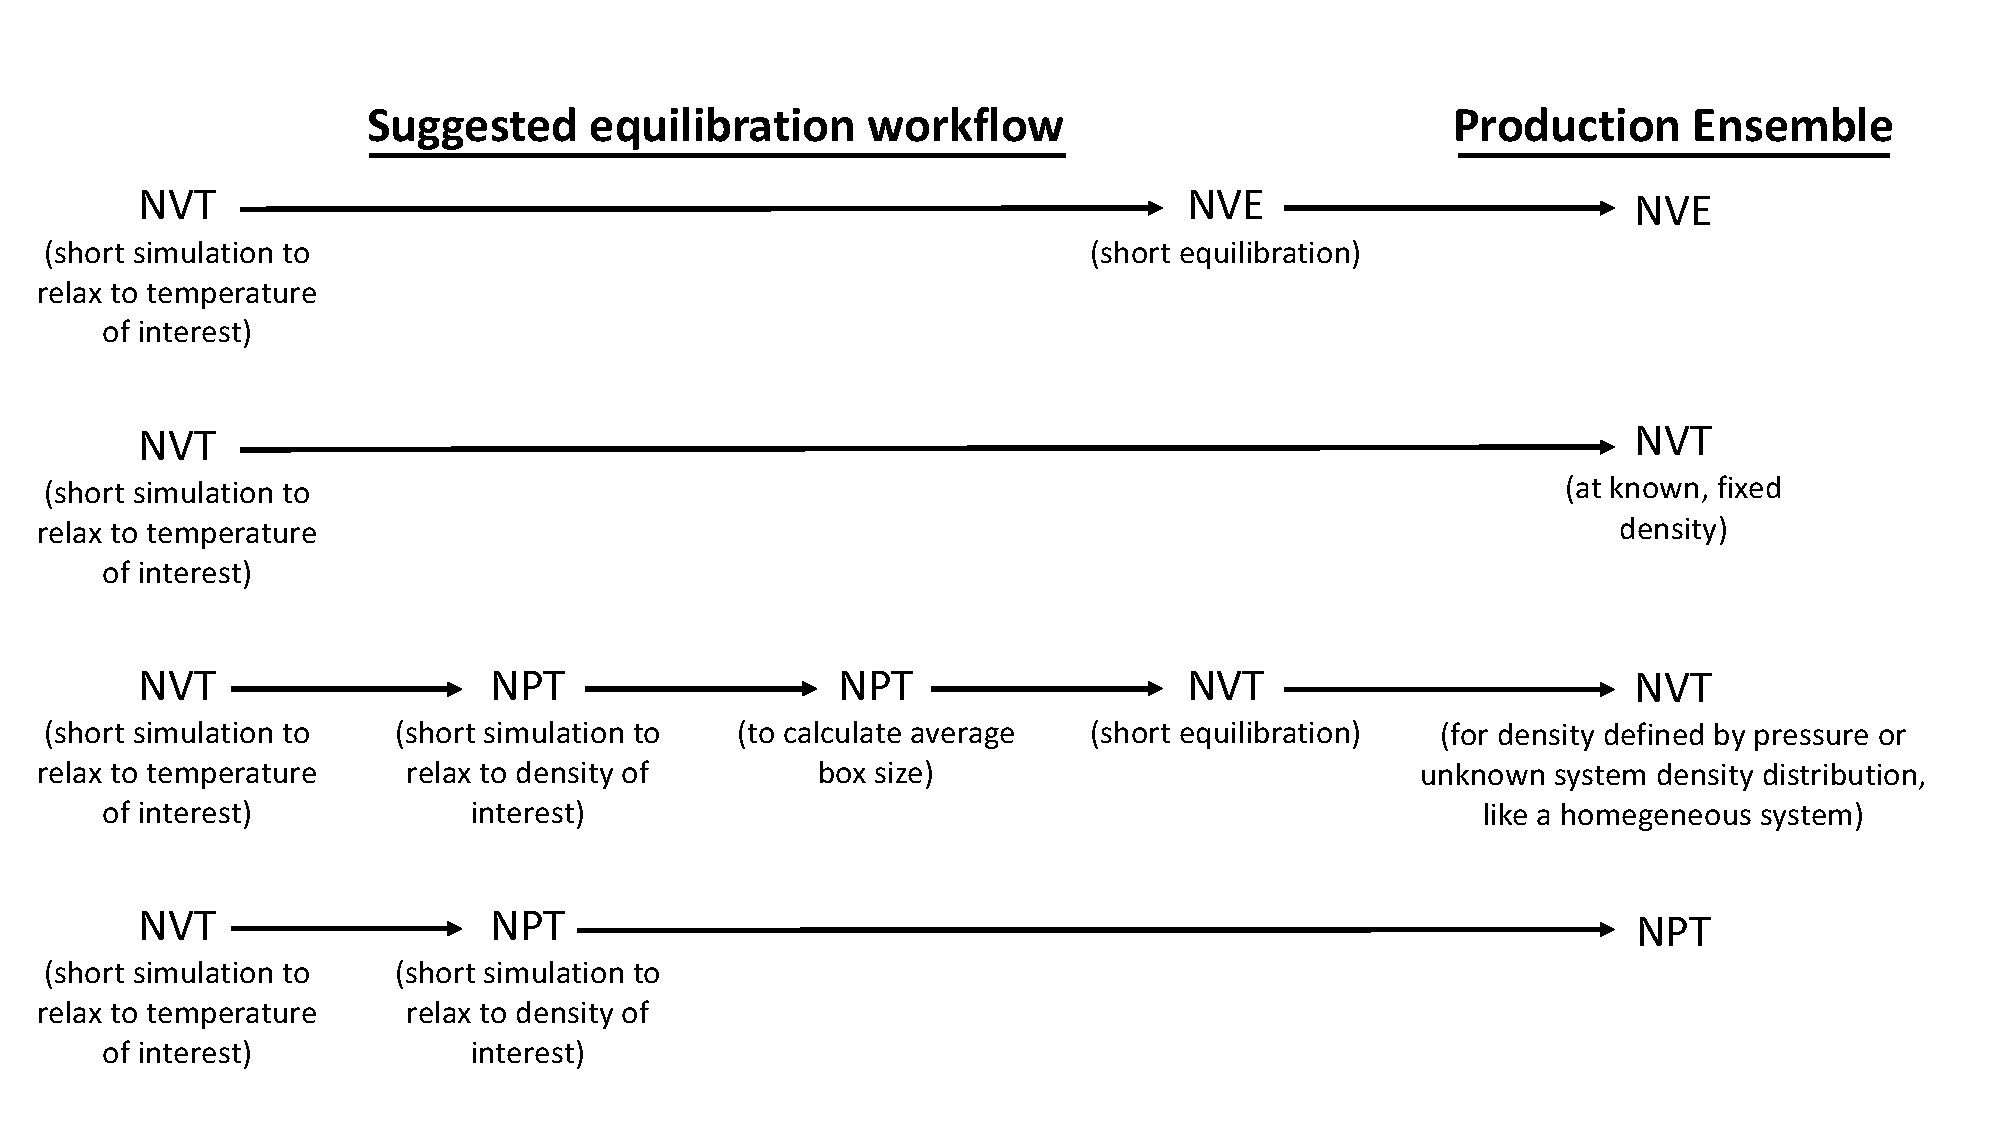
\includegraphics[width=\linewidth]{Equilibration_Workflow.pdf}
\caption{Common equilibration work-flows}
\label{eqworkflow}
\end{figure}

Once equilibration is complete, the production simulation may be performed. 
The production simulation is that from which specific properties of the system of interest will be calculated. 
As mentioned above, the equilibration procedure should be selected that is appropriate for the desired production ensemble. 
It should be noted that "equilibration" within the production run may still be necessary before properties or metrics are computed from this simulation (see \citet{ShellNotes}, lecture on Computing properties). 
This falls under the category of correctly obtaining unbiased statistics and convergence, which is covered in another best-practices document. %How to cite? Do we even cite this? 
Otherwise, if a brief simulation in the same ensemble is not performed during the equilibration step immediately prior to production, any period of the production simulation should be ignored where drift is observed in the energies, temperatures, pressures, densities, or other defining state-variables of the ensemble. 
This of course proceeds estimation of convergence in property calculation.
For more specific details on procedures and parameters used in production simulations, see the appropriate best practices document for the system of interest.

\subsection{Thermostats}
\begin{itemize}
\item What is it?
\item Brief description of how it works
\item Popular thermostats
\end{itemize}

\subsection{Barostats}
\begin{itemize}
\item What is it?
\item Brief description of how it works
\item Popular thermostats
\end{itemize}

\subsection{Integrators}
\begin{itemize}
\item Numerical solution of dynamical equations of motions
\item Importance of energy conservation
\item Commonly used integrators
\item How to choose an appropriate timestep?
\end{itemize}

\subsection{Long range electrostatics}
\begin{itemize}
\item Cut-off is bad
\item Need for special treatment
\item Idea of an Ewald sum
\item PPPM 
\item How to choose parameters
\end{itemize}

\section{Checklist}
\begin{itemize}
\item \textbf{Count the cost:} Think about what you know about the timescales of what you want to observe and determine whether it is tractable to simulate this given the size of your system, your computational resources, and the expense of the simulation.
\item Pick the desired ensemble ($NVT$, $NPT$, $NVE$, $\mu VT$, $\mu PT$)
\item Determine reference states that you are trying to emulate/discover.
\begin{itemize}
\item What Temp, pressure, etc.
\item What values in experimental
\item What values in literature?
\end{itemize}
\item Choose a simulation package suitable for simulating that ensemble (see best practices document) 
\item Determine whether you are simulating a bulk (typically periodic) or finite system and choose the appropriate cutoffs and periodicity (full periodicity for bulk systems, partial periodicity for interfaces, etc.)
\begin{itemize}
\item As a general rule, electrostatics are long-range enough that either the cutoff needs to be larger than the system size (for finite systems) or periodicity is needed
\item Nonpolar interactions can often be safely treated with cutoffs of 1-1.5 nm as long as the system size is at least twice that, but long-range dispersion corrections may be needed
\end{itemize}
\item Choose appropriate settings for the ensemble:
\begin{itemize}
\item Pick a thermostat that gives the correct distribution of temperatures, not just the correct average temperature
\item Pick a barostat that gives the correct distribution of pressures
\end{itemize}
\item Choose an appropriate timestep for stability and avoiding energy drift
\begin{itemize}
\item This depends on factors such as the use of constraints in the system (e.g. for all-atom systems constraining hydrogen bonds can allow the use of a slightly longer timestep; 2 fs is relatively typical)
\item If your initial structure is potentially strained, energy minimize before starting
\item The shortcomings and limitations of certain integrators and thermostats/barostats
\begin{itemize}
\item Ergodicity issue with non-chained Nose-Hoover
\item Error that is propagated with integrators in terms of dt
\end{itemize}
\end{itemize}
\end{itemize}






\nocite{*}
\bibliography{basic_training}{}

\end{document}
